\section{Question 1}
     \subsection{Tìm tọa độ, diện tích, chu vi, góc (độ) của hình sử dụng image moment và lập trình so sánh với hàm OpenCV}
          \subsubsection{Tính tay sử dụng image moment}
               \hspace*{0.6cm}Hình có ma trận sau:
               \begin{table}[h]
                    \centering
                    \begin{tabular}{|c|c|c|c|c|c|c|}
                    \hline
                    0 & 0 & 0 & 0 & 0 & 0 & 0 \\ \hline
                    0 & 0 & 0 & 255 & 0 & 0 & 0 \\ \hline
                    0 & 0 & 255 & 255 & 255 & 0 & 0 \\ \hline
                    0 & 255 & 255 & 255 & 255 & 255 & 0 \\ \hline
                    0 & 255 & 255 & 255 & 255 & 255 & 0 \\ \hline
                    255 & 255 & 0 & 0 & 0 & 255 & 255 \\ \hline
                    0 & 0 & 0 & 0 & 0 & 0 & 0 \\ \hline
                    \end{tabular}
               \end{table}
               \begin{itemize}
                    \item \textbf{Tọa độ tâm của hình và diện tích}
                    \newline
                    \hspace*{0.6cm}Công thức tổng quát moment của ảnh
                    \begin{equation}
                         M_{p,q} = \sum_{i} \sum_{j} i^p j^q I(i,j) 
                         \label{eq:s1_eq1}
                    \end{equation}                    
                    \hspace*{0.6cm}Tọa độ tâm của ảnh được tính bằng công thức
                    \begin{align}
                         &x_c = \dfrac{M_{1,0}}{M_{0,0}} \label{eq:s1_eq2}\\
                         &y_c = \dfrac{M_{0,1}}{M_{0,0}} \label{eq:s1_eq3}
                    \end{align}    
                    \hspace*{0.6cm}Ta có
                    \begin{align*}
                         M_{0,0} &= \sum_{i} \sum_{j} I(i,j) = 1 \times 18 = 18\\
                         M_{1,0} &= \sum_{i} \sum_{j} i \cdot I(i,j) \\
                                 &= 1 \times (0 \times 1 + 1 \times 3 + 2 \times 3 + 3 \times 4 + 4 \times 3 + 5 \times 3 + 6 \times 1) = 54\\
                         M_{0,1} &= \sum_{i} \sum_{j} j \cdot I(i,j) \\
                                 &= 1 \times (0 \times 0 + 1 \times 1 + 2 \times 3 + 3 \times 5 + 4 \times 5 + 5 \times 4 + 6 \times 0) = 62
                    \end{align*}
                    \hspace*{0.6cm}Suy ra
                    \begin{align*}
                         &S = M_{0,0} = 18\\
                         &x_c = \dfrac{54}{18} = 3\\
                         &y_c = \dfrac{62}{18} = 3.4444 \approx 3
                    \end{align*}
                    \item \textbf{Chu vi}
                    \newline
                    \hspace*{0.6cm}Contour của hình và loại pixel thể hiện trong hình
                    \begin{table}[h]
                         \centering
                         \begin{tabular}{|c|c|c|c|c|c|c|}
                         \hline
                         0 & 0 & 0 & 0 & 0 & 0 & 0 \\ \hline
                         0 & 0 & 0 & b & 0 & 0 & 0 \\ \hline
                         0 & 0 & b & 0 & b & 0 & 0 \\ \hline
                         0 & c & 0 & 0 & 0 & c & 0 \\ \hline
                         0 & c & c & a & c & c & 0 \\ \hline
                         c & c & 0 & 0 & 0 & c & c \\ \hline
                         0 & 0 & 0 & 0 & 0 & 0 & 0 \\ \hline
                         \end{tabular}
                    \end{table}
                    \newline
                    \hspace*{0.6cm}Chu vi của hình được tính bằng
                    \begin{equation*}
                         P = n(a) + n(b)\sqrt{2} + n(c) \dfrac{1+\sqrt{2}}{2}
                    \end{equation*}
                    \hspace*{0.6cm}Trong đó $n(a), \, n(b), \, n(c)$ lần lượt là số lượng pixel loại a, b, c.
                    \newline
                    \hspace*{0.6cm}Vậy ta có
                    \begin{equation*}
                         P = 1 + 3 \times \sqrt{2} + 10 \times \dfrac{1+\sqrt{2}}{2} \approx 17.3137
                    \end{equation*}
                    \item \textbf{Góc của hình (độ)}
                    \newline
                    \hspace*{0.6cm}Góc xoay của hình được tính bằng công thức
                    \begin{align}
                         \theta = \dfrac{1}{2} \arctan \left( \dfrac{2 \mu_{11}^{'}}{\mu_{20}^{'} - \mu_{02}^{'}} \right)
                         \label{eq:s1_eq4}
                    \end{align}
                    \hspace*{0.6cm}Trong đó 
                    \begin{align*}
                         &\mu_{11}^{'} = \dfrac{M_{1,1}}{M_{0,0}} - x_c y_c\\
                         &\mu_{20}^{'} = \dfrac{M_{2,0}}{M_{0,0}} - x_c^2\\
                         &\mu_{02}^{'} = \dfrac{M_{0,2}}{M_{0,0}} - y_c^2
                    \end{align*}
                    \hspace*{0.6cm}Lần lượt tính các moment cần thiết
                    \begin{align*}
                         M_{1,1} = \sum_{i} \sum_{j} i j I(i,j) &= 0 + 1 \times (3 + 4 + 5) + 2 \times (2 + 3 + 4) + 3 \times (1 + 2 + 3 + 4)\\
                                   & + 4 \times (2 + 3 + 4) + 5 \times (3 + 4 + 5) + 6 \times 5 = 186
                    \end{align*}
                    \begin{equation*}
                         M_{2,0} = \sum_{i} \sum_{j} i^2 I(i,j) = 0 + 1^2 \times 3 + 2^2 \times 3 + 3^2 \times 4 + 4^2 \times 3 + 5^2 \times 3 + 6^2 \times 1 = 210                    
                    \end{equation*}
                    \begin{equation*}
                         M_{0,2} = \sum_{i} \sum_{j} j^2 I(i,j) = 0 + 1^2 \times 1 + 2^2 \times 3 + 3^2 \times 5 + 4^2 \times 5 + 5^2 \times 4 + 6^2 \times 0 = 238          
                    \end{equation*}
                    \hspace*{0.6cm}Suy ra
                    \begin{align*}
                         &\mu_{11}^{'} = \dfrac{186}{18} - 3 \times \dfrac{62}{18} = 0\\
                         &\mu_{20}^{'} = \dfrac{210}{18} - 3^2 = \dfrac{8}{3} \approx 2.67\\
                         &\mu_{02}^{'} = \dfrac{238}{18} - \left( \dfrac{62}{18} \right)^2 = \dfrac{110}{18} \approx 1.358
                    \end{align*}
                    \hspace*{0.6cm}Thay vào công thức \ref{eq:s1_eq4} ta có
                    \begin{equation*}
                         \theta = \dfrac{1}{2} \arctan \left( \dfrac{2 \times 0}{2.67 - 1.358} \right) = 0^{\circ}
                    \end{equation*}
                    \item \textbf{Kết luận}
                    \newline
                    \hspace*{0.6cm}Các giá trị tính toán tay theo yêu cầu đề bài như sau:
                    \begin{itemize}[label={--}]
                         \item Tọa độ tâm: $(3, 3.444) \approx (3, 3)$
                         \item Diện tích: 18 pixel
                         \item Chu vi: $\approx$ 17.3137
                         \item Góc: 0$^{\circ}$
                    \end{itemize}
               \end{itemize}
          \subsubsection{Lập trình kiểm tra và so sánh với kết quả sử dụng hàm OpenCV}
               \hspace*{0.6cm}Đoạn code lập trình kiểm tra kết quả tính toán
               \begin{lstlisting}
ys, xs = np.where(img == 255)
M00 = len(xs)
M10 = np.sum(xs)
M01 = np.sum(ys)
M11 = np.sum(xs * ys)
M20 = np.sum(xs**2)
M02 = np.sum(ys**2)
x_centroid = M10 / M00
y_centroid = M01 / M00
u11 = M11 / M00 - x_centroid * y_centroid
u20 = M20 / M00 - x_centroid**2
u02 = M02 / M00 - y_centroid**2
theta = 0.5 * np.arctan2(2 * u11, u20 - u02)  # in radians
print("M00: ", M00, " M10: ", M10, " M01: ", M01)
print("M11 = ", M11, " M20 = ", M20, " M02 = ", M02)
print("Area: ", M00, " pixels")
print("Centroid: ", (x_centroid, y_centroid), "approx", (int(x_centroid), int(y_centroid)))
print("Orientation angle (degrees): ", np.degrees(theta))
               \end{lstlisting}
               \hspace*{0.6cm}Kết quả
               \begin{figure}[H]
                    \centering
                    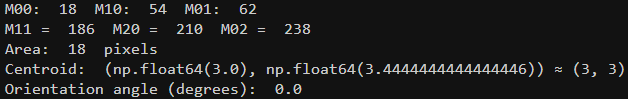
\includegraphics[width=1\textwidth]{pictures/chapter1/c01_p01_result_1a_1.png}
                    \caption{Kết quả lập trình tính toán các thông số}
                    \label{s1_p01}
               \end{figure}
               \hspace*{0.6cm}Đoạn code sử dụng hàm OpenCV để kiểm tra kết quả
               \begin{lstlisting}
contours, _ = cv2.findContours(img, cv2.RETR_LIST, cv2.CHAIN_APPROX_SIMPLE)
for contour in contours:
    # Centroid
    M = cv2.moments(contour)
    if M["m00"] != 0:
        cx = int(M["m10"] / M["m00"])
        cy = int(M["m01"] / M["m00"])
        print(f"Centroid: ({cx}, {cy})")
    
    # Area
    area = cv2.contourArea(contour)
    print(f"Area: {area}")
    
    # Perimeter
    perimeter = cv2.arcLength(contour, True)
    print(f"Perimeter: {perimeter}")
    
    # Orientation 
    if len(contour) >= 5:  
        ellipse = cv2.fitEllipse(contour)
        angle = ellipse[2]
        print(f"Orientation angle: {angle} degrees")
               \end{lstlisting}
               \hspace*{0.6cm}Kết quả
               \begin{figure}[H]
                    \centering
                    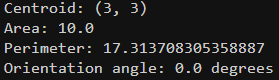
\includegraphics[width=0.5\textwidth]{pictures/chapter1/c01_p01_result_1a_2.png}
                    \caption{Kết quả sử dụng hàm OpenCV để kiểm tra}
                    \label{s1_p02}
               \end{figure}

